\section{Test Beam Setup}

SiPMs are one of the main features of new electronics that are being installed in the CMS detector. These new readout modules main function is to take the signals from the detector, the light signals from incident particles and convert them to digitized charge signals which can be later stored and analyzed. There are several new features with these new readout modules such as new charge integrator and encoder (QIE) chips, but the main subject of my work was the SiPMs. The main way the SiPM non-linearity and other things about the new readout modules are being study is with a test beam. The test beam is a linear particle beam that comes from the SPS accelerator when it does not feed into the LHC. The particles from this beam are not at the energies of the protons in the LHC but they are much easier to make and control. There are several different experiments that use this beam but the HCAL has a mock test stand that can be moved into the path of the beam when experiments need to be run. The CMS detector is 100 meters underground and is in a cavern that due to radiation and tight enclosures makes the detector difficult to access. Though modifications and maintenance can be during shutdowns this is not the ideal way to run tests on new electronics. The test stand at the test beam location called H2 can be easily accessed observed and is on ground level. In addition the energy and particle type of the beam can be easily controlled. The test stand is designed to be similar to a portion of the HCAL on CMS. As such when we shoot particles from the test beam at the test stand with the new electronics on it we can measure its response to experiment like conditions. Using this test beam we can shoot particles like pions at the test stand which has the new readout module installed and look at the response. We can vary the energy of the pions which should increase the number of incident photons on the SiPMs in the readout modules and measure their response to this. In this way we can find the non-linearity of the SiPMs and create a correction curve based on this.

Because we are looking for statistical in the data we need to take a lot of data. This means we take runs with several thousand events or particle hitting the test stand and take several of these runs to ensure high statistics. On the other hand this means we want o minimize the amount of information stores per event so we can store a lot of them. One of the key systems that helps this is the trigger system. In the path of the beam before the test stand we put scintillator tiles not designed to stop the particle entire but rather to send a generic signal to the control room. A total of four tiles were placed in the path of the beam. When we saw signals from these tiles we know that a particle is coming from the beam. This serves as our trigger signal. The trigger signal then goes to the back-end electronics that stores the data from the detector. In this way we only store data coming during the short amount of time on the order of 25 nanoseconds when we know their is relevant information coming. There is also a ready signal that goes from the back-end electronics to the trigger. Since a particle may come before the back-end electronics are finished storing the relevant data a trigger signal that comes without the ready signal will simply be ignored.

Although built to be similar to the HCAL on the CMS detector the test stand is smaller and has some differences. When looking at the data from the teat beam it is important to be sure that the e-map, which traces the channels that receive the data to the actual scintillator tiles on the detector, is correct. To account for the difference between the test stand and the HCAL a new e-map needed to be created. With an accurate e-map we can create an accurate picture of the incident particles hitting the test stand. The test beam allows us to control the energy and type of particles incident on the test stand. This allows us to study things like SiPM non-linearity as we can look at the output of the SiPMs under something like $50 \GeV$ pions then increase to energy to something like $150 \GeV$ and compare the different responses. However the particle does not deposit its energy in a single scintillator tile. For something like a pion it will lose a part of its energy with each scintillator tile it hits and eventually be stopped by the detector but its total energy will be spread throughout the detector. Since each particle in the beam has roughly the same energy and we can isolate the event of a single particle hitting the detector we are to find energy lost in each scintillator tile but looking at the complete picture of the detector. 

SiPM non-linearity is not the only thing that is being researched using the test beam. In the CMS detector particles come so fast that the signals of individual particles blend together. In the test beam the particles are more spread out so it is easier to isolate the signal of individual particles. This makes it easier to extract the pulse shape of the readout modules which is the shape of the output charge vs time. It is also important to see if the pulse shape changes significantly under different circumstances such as higher or lower energies. Using the pulse shape of the readout modules we can then extract the individual signals in the CMS detector.

\section{Test Beam Analysis}

With a proper e-map we can get a picture of the incident particle and observe its path and where it deposited its energy. Since the particle does not deposit all of its energy in a single scintillator tile this is critical when trying to recreate the particle energy. It is also important that there are often a variable amount of scintillator tiles in a single depth channel as shown in figure~\ref{fig:emap} which shows 4 scintillator tiles in depth 5 and 3 scintillator tiles in depth 4. Looking at the results in the plot to the left it explains why there is more energy deposited in depth 5 rather than depth 4. 

\begin{figure}
\centering
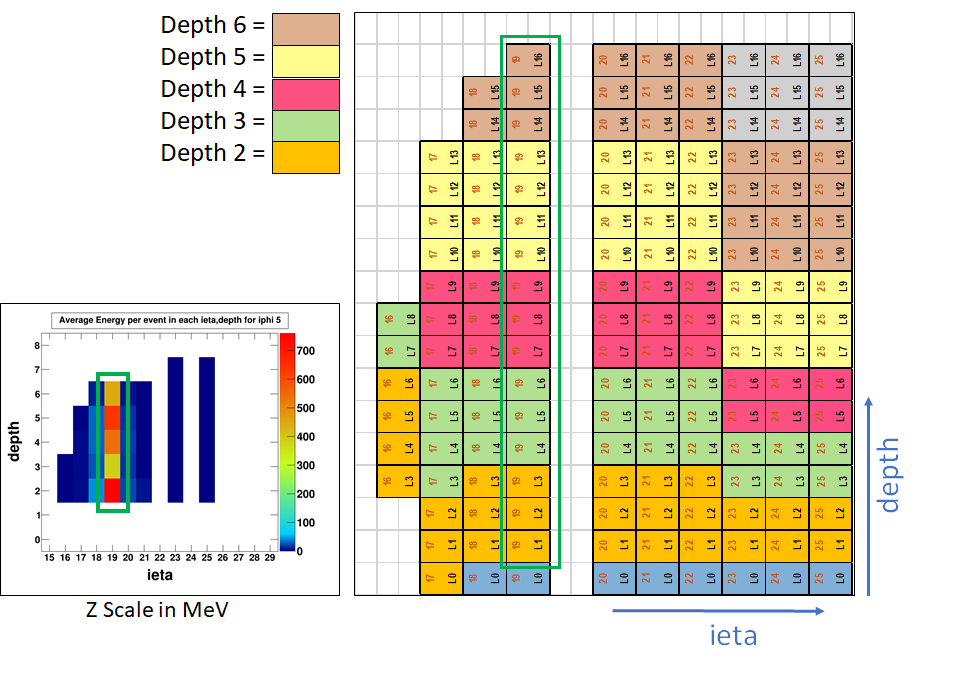
\includegraphics[width=\linewidth]{Figures/eplot.png}
\caption{This shows the relationship between the emap on the left showing which contains a geometric layout of the scintillator tiles in a single iphi slice and the data plots in a run with 150 GeV muons.}
\label{fig:emap}
\end{figure}

Muons are useful for many things but when trying to recreate the energy of the particle it is easier to use pions. The reason for this is that muons tend to go through the detector depositing a small portion of the energy but not being entirely stopped. This can be seen in figure~\ref{fig:emap} which shows the muons depositing a consistent amount of energy in each of the depths even the far ones. One the other hand figure~\ref{fig:pionmap} shows a similar plots with a pion run. This shows that the pions hit the scintillator tiles in depth 2 depositing a large portion of their energy and depositing less and less in the next depths with basically nothing in the last depth. There is also more significant spread compared to the muon run which shows the muons going straight through while the pions leave some energy in the neighboring channels.

\begin{figure}
\centering
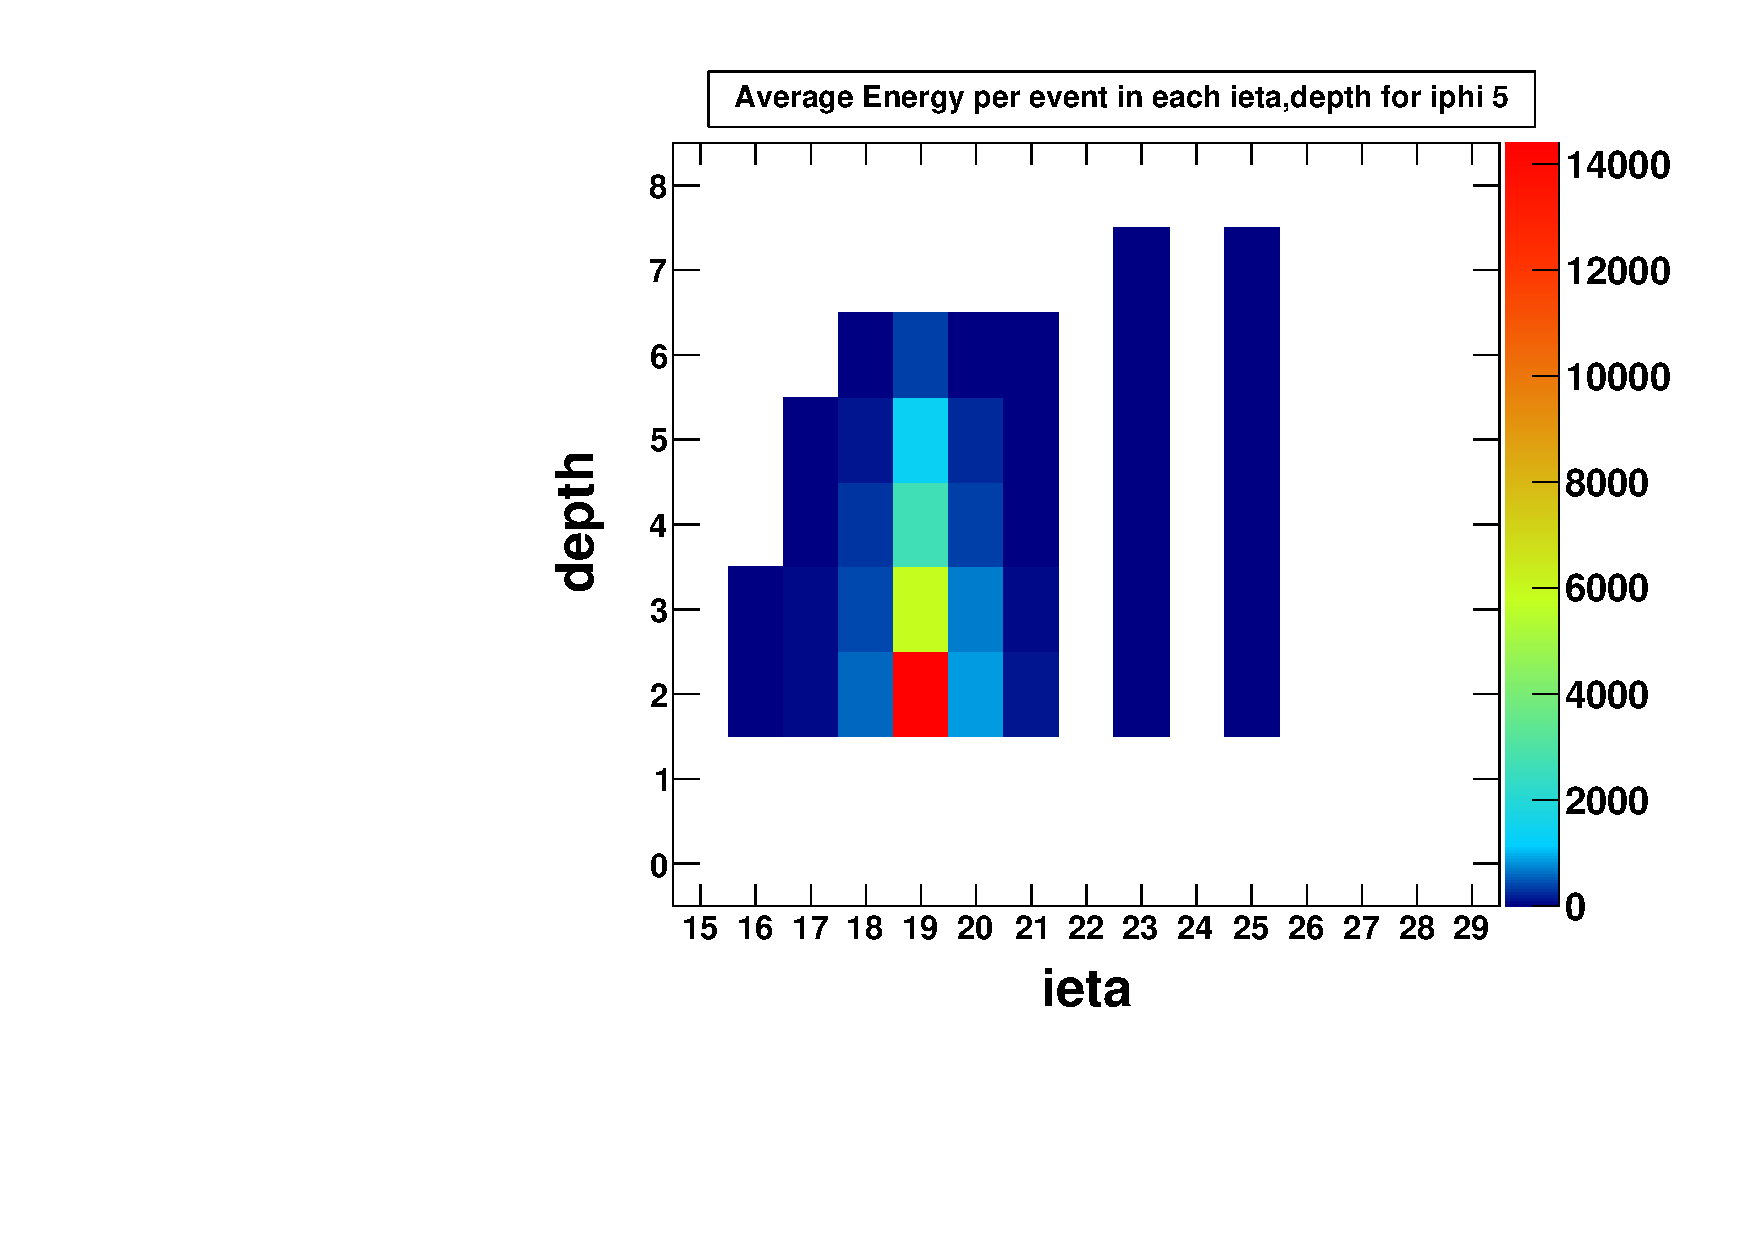
\includegraphics[width=0.7\linewidth]{Figures/pionrun.pdf}
\caption{This shows the recreation of an event with 50GeV pions showing the pions aimed at iphi 5 ieta 19 and the energy deposited in each channel z scale in MeV.}
\label{fig:pionmap}
\end{figure}

To recreate the energy of the incident particle we can look at plots such as figure~\ref{fig:pioncharge} which shows the mean output charge in a 50GeV pion run. By looking at this output charge and the output charge of the other channels we can find what portion of the particles energy was deposited in this channel and then going by the known energy of the particle how much energy was deposited to produce this output charge. 

\begin{figure}
\centering
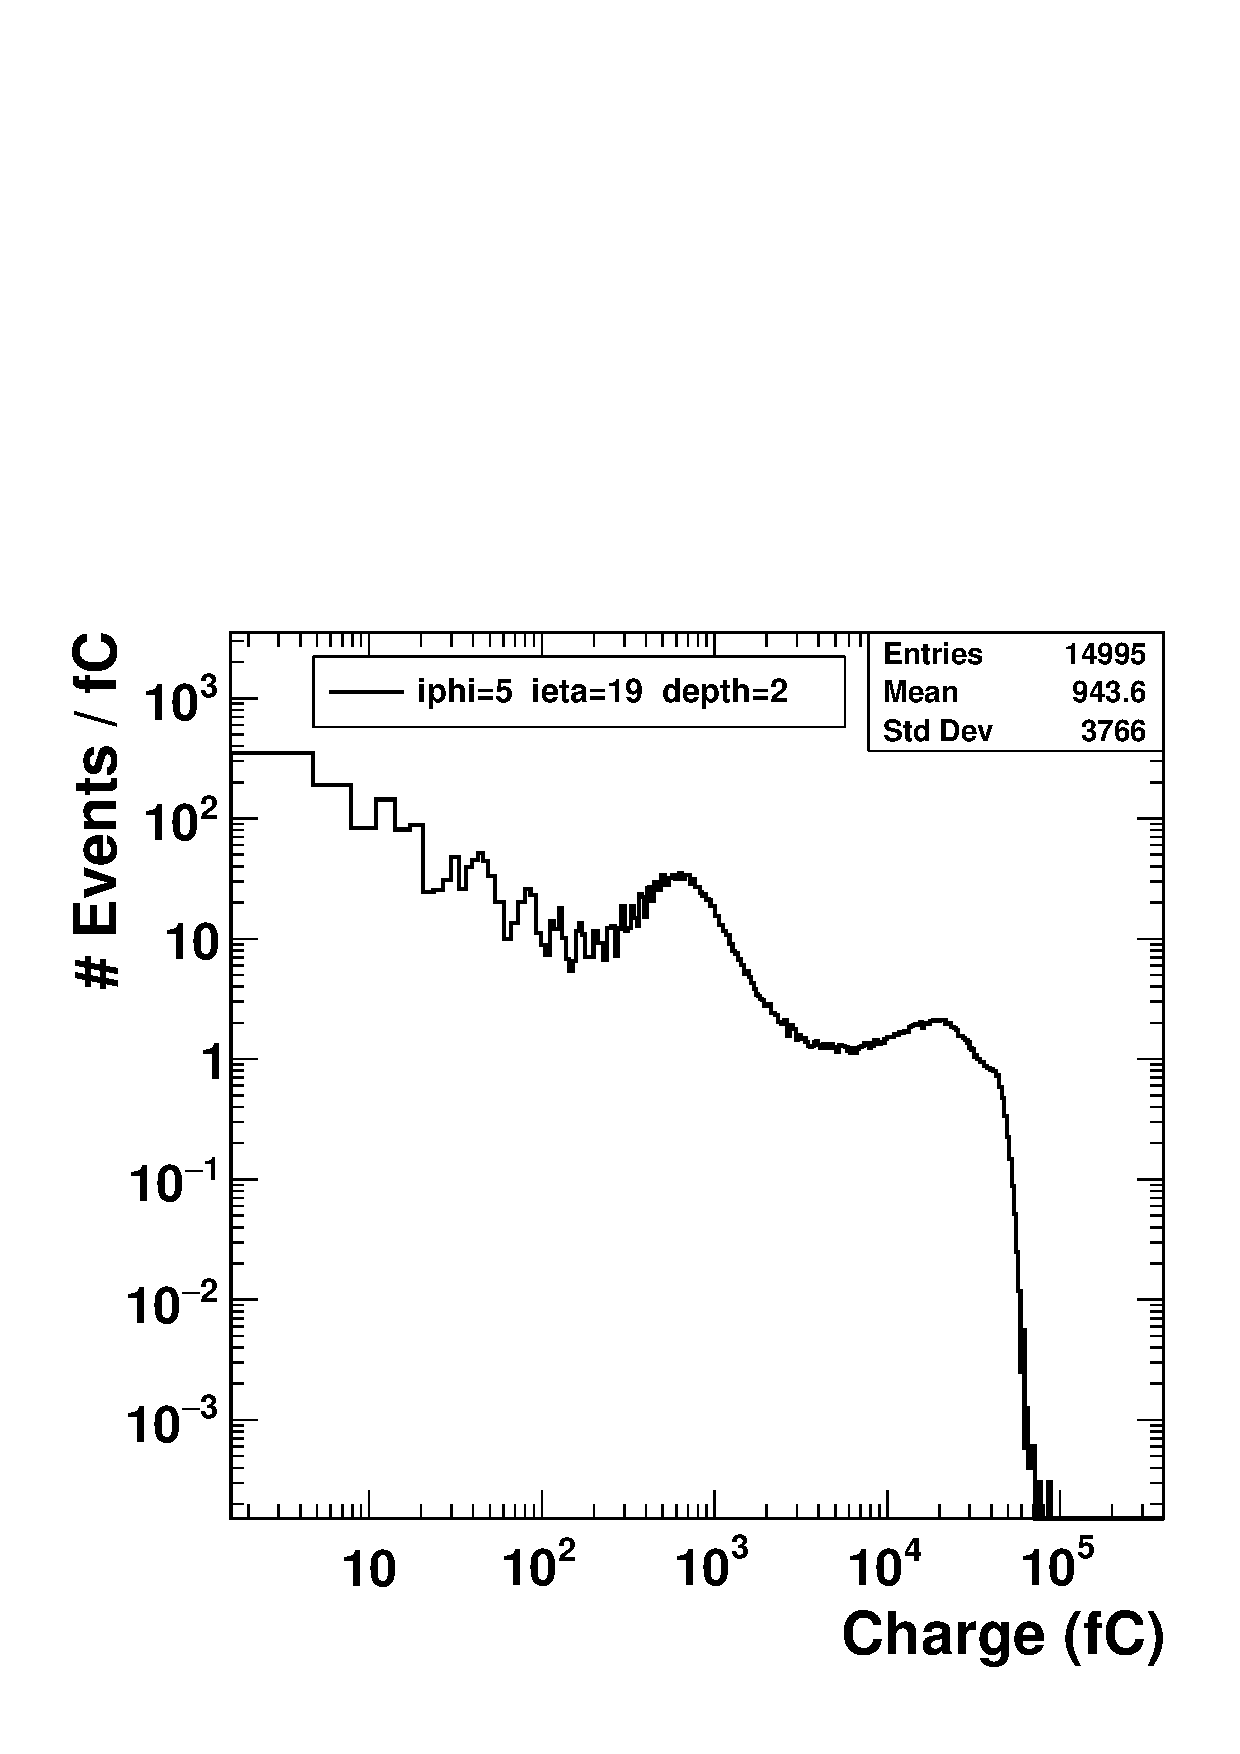
\includegraphics[width=0.7\linewidth]{Figures/pioncharge.pdf}
\caption{This shows the number of events that produces output charge in the SiPM. The peak in the middle shows the average output charge in response to the incident particles at this energy.}
\label{fig:pioncharge}
\end{figure}

%This is the pion run I used for the timing information. Would it be better to use a higher energy pion run?

One of the key things in doing a pulse shape analysis using test beam data is the timing information. In the test beam we take two different timing information. The first comes from the QIE chips in the readout modules. The readout modules measure the output charge of the SiPM over 250ns and the information is binned into 10 time samples each 25ns long. The output pulse of the SiPM is about 75ns long so it usually stays confined to 3 or 4 time samples. In addition we also take what is called a Time to Digital Converter (TDC) value. This value stores at what time in the 250ns span the output charge of the SiPM crossed a threshold with a 0.5ns resolution. Since the output charge starts out below this threshold, the TDC value should give the the start of the output pulse of the SiPM. One of the problems with the TDC value is that it could be affected by the amplitude of the output pulse as a high amplitude will cross this threshold earlier. To extract the pulse shape we can do something called a phase scan. In a phase scan we delay starting the taking of data by something less than 25ns. Since the pulse does not come in in time sample 0 we do not loose any of the pulse but simply move parts of the output pulse into different time samples. By doing this we can extract the pulse shape with a resolution much greater than 25ns. 

\begin{figure}
\centering
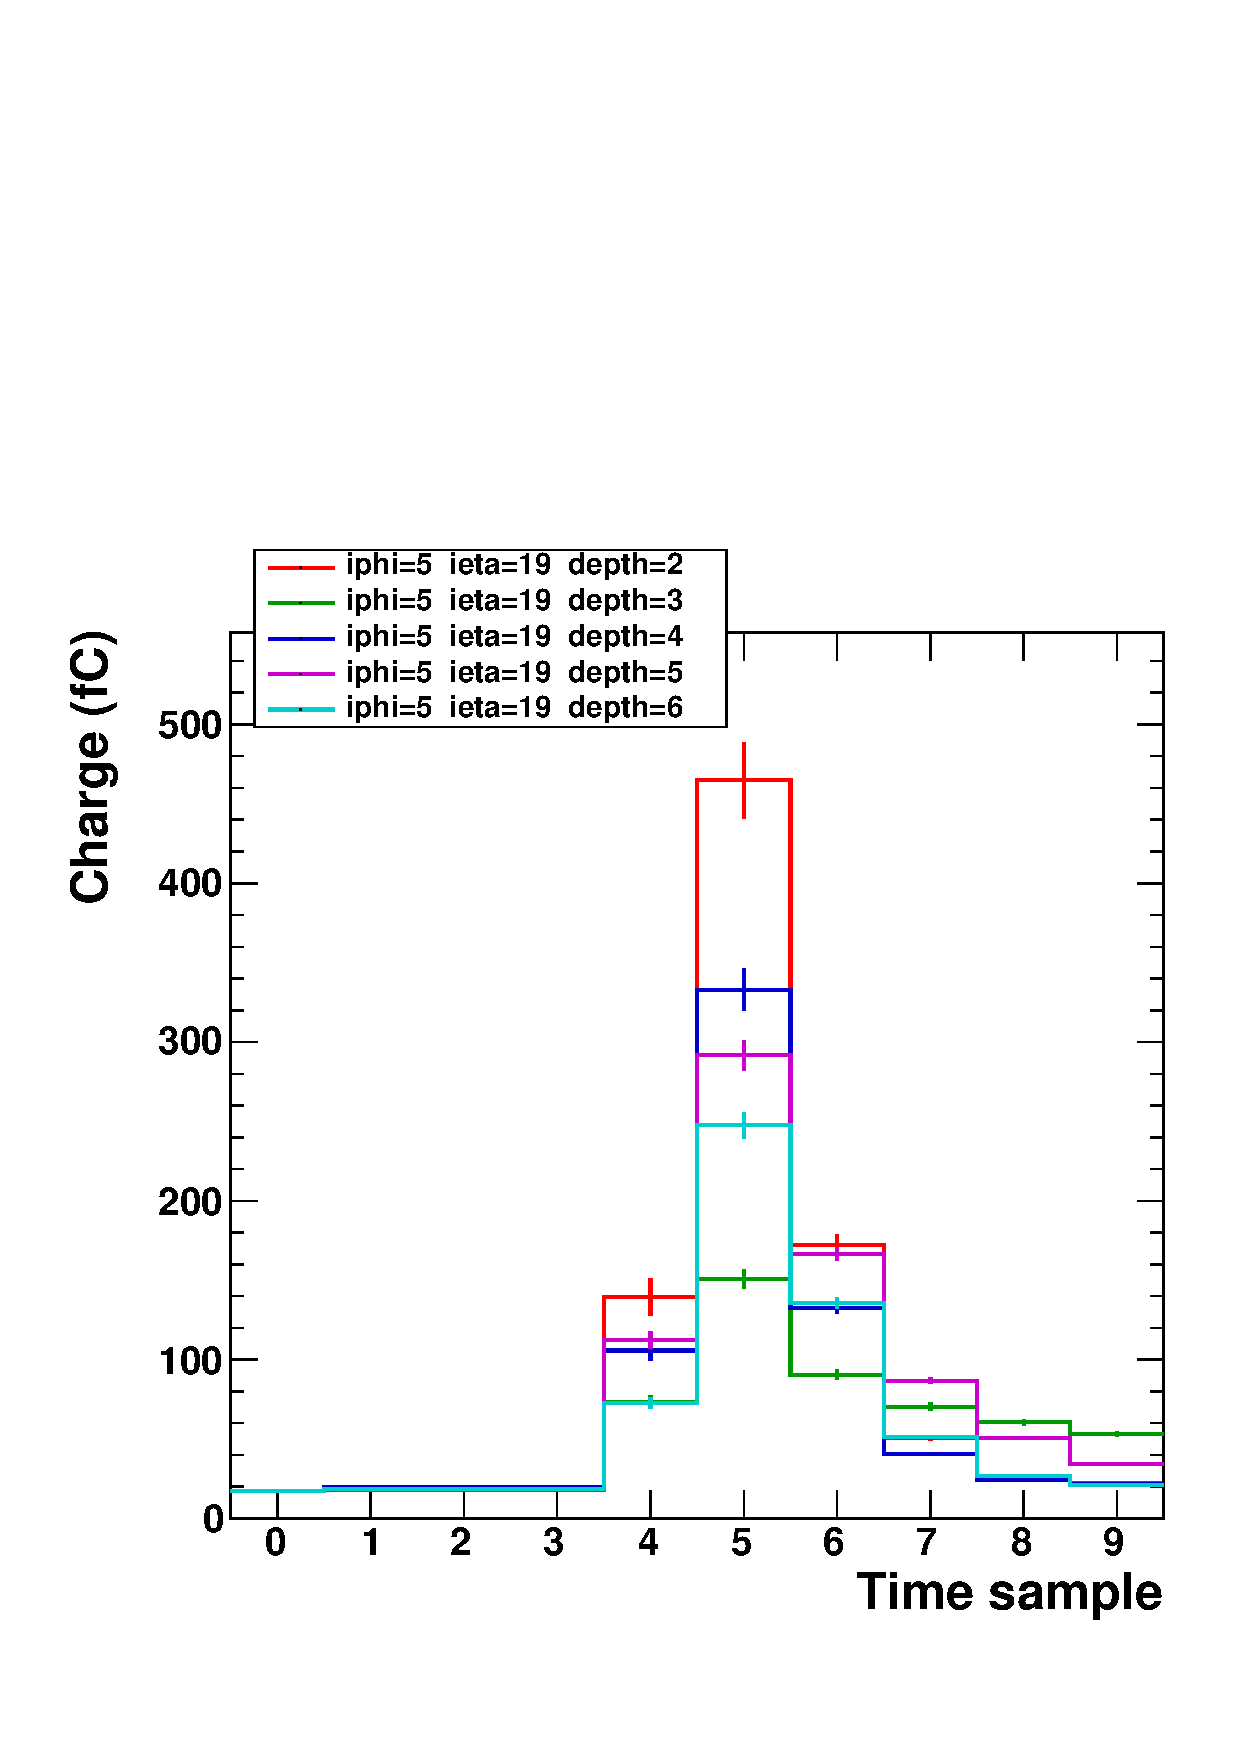
\includegraphics[width=0.7\linewidth]{Figures/Pulse.pdf}
\caption{A histogram of the output pulse of the readout modules binned in 25ns bins. This is from a run with 150GeV muons aimed at iphi5 and ieta 19. This plot shows the output pulse of the different depths at that location.}
\label{fig:PulSh}
\end{figure}

There is also the trigger information. This timing information comes from the test beam equipment that signals the back end electronics to store the data from the readout modules. The trigger information theoretically does not have the same discrepancy as TDC information but most people still use the TDC from the QIE chips. The relationship between the two signals can be shown in figure~\ref{fig:tdc}.

\begin{figure}
\centering
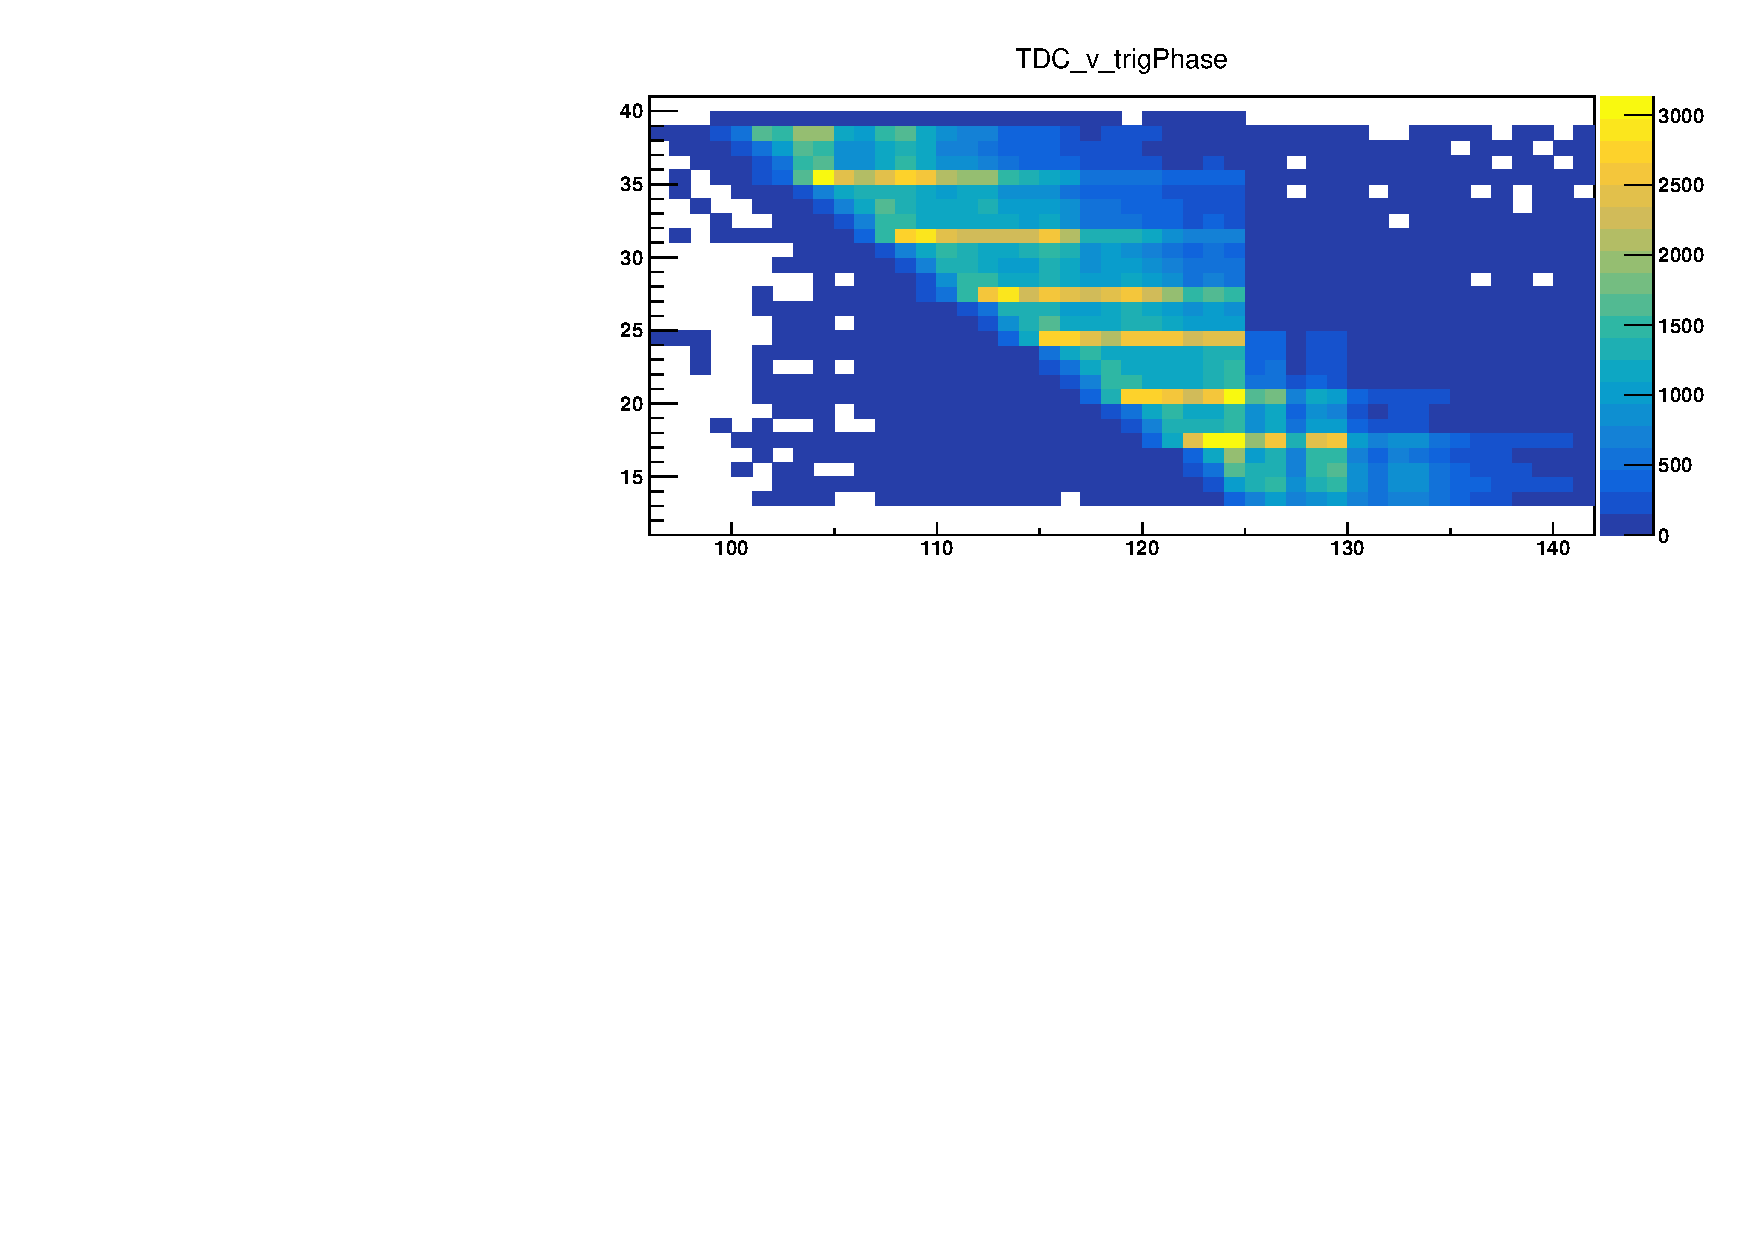
\includegraphics[width=\linewidth]{Figures/zoom.pdf}
\caption{A histogram showing the statistical relationship between the trigger timing information and the QIE TDC information.}
\label{fig:tdc}
\end{figure}

%I think I have a good idea of what is going in these plots and testbeam itself but I am lacking in actual analysis results. I guess may main question at this point is how do we get from these plots to things like a non-linear correction curve or a pulse shape.

